\documentclass[]{article}
\usepackage[a4paper, margin=2cm]{geometry}
\usepackage{amsmath}
\usepackage{amsfonts}
\usepackage{amssymb}
\usepackage{mathtools}
\usepackage{amsthm}
\usepackage[many]{tcolorbox}
\usepackage{listings}
\usepackage{cancel}
\usepackage{graphicx}
\usepackage{subfigure}

\newtheorem{lemma}{Lemma}
\newtheorem{theorem}{Theorem}
\newtheorem{definition}{Definition}
\newtheorem{algorithm}{Algorithm}
\newtheorem{example}{Example}
\newtheorem{remark}{Remark}
\newtheorem{recap}{Recap}
\newtheorem{corollary}{Corollary}


\tcolorboxenvironment{lemma}{
	colback=yellow!5!white,
	boxrule=0pt,
	boxsep=1pt,
	left=2pt,right=2pt,top=2pt,bottom=2pt,
	oversize=2pt,
	sharp corners,
	before skip=\topsep,
	after skip=\topsep,
}

\tcolorboxenvironment{definition}{
	colback=green!5!white,
	boxrule=0pt,
	boxsep=1pt,
	left=2pt,right=2pt,top=2pt,bottom=2pt,
	oversize=2pt,
	sharp corners,
	before skip=\topsep,
	after skip=\topsep,
}
\begin{document}
	
	\title{Computer Aided Geometric Design Compendium WS2023}
	\author{Ida Hönigmann}
	
	\maketitle

\section*{Organization}
Lecture each Thursday 12:00 to 14:00 (full 2 hours).
\\
Oral exam. Write email to fix date and time.
\\
Problem session each Thursday 14:00 to 16:00. Mandatory attendance!
\\
Kreuzerlübung.

\section{Bezier curves}

\begin{example}
	\begin{figure}[h!]
		\subfigure{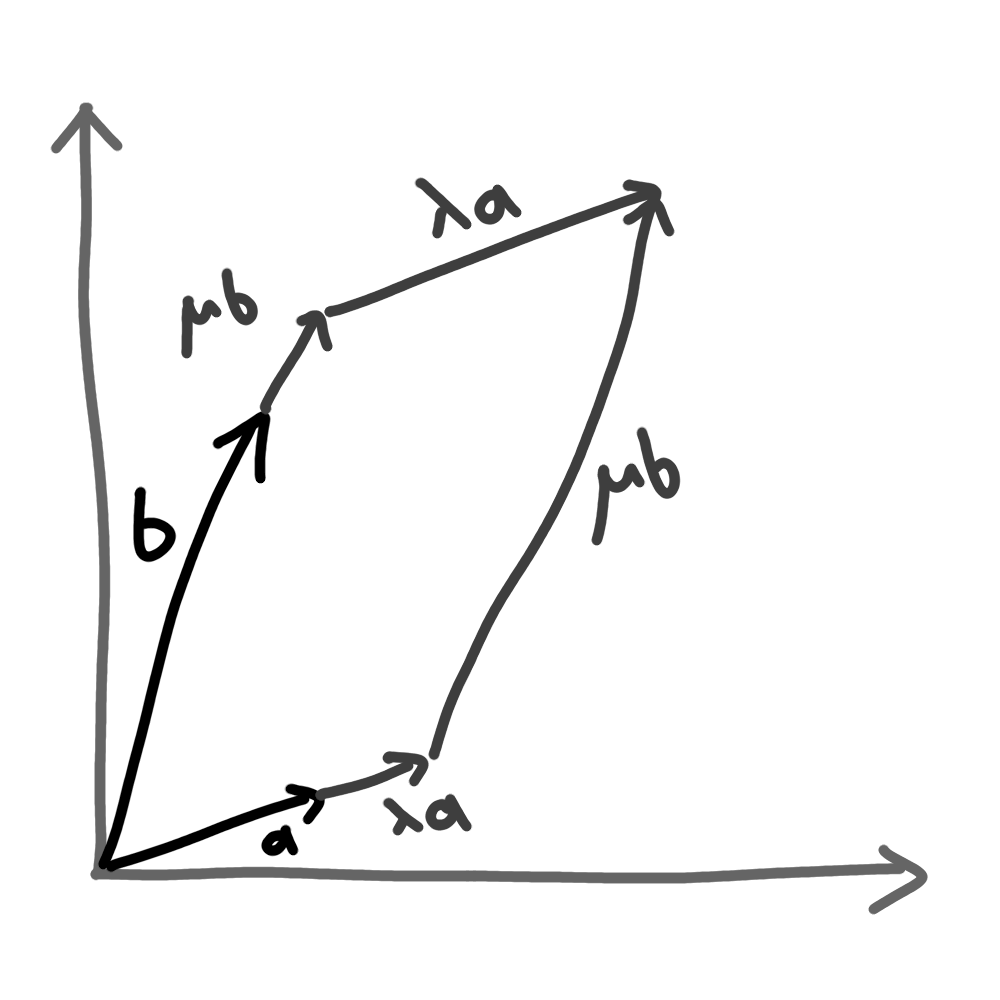
\includegraphics[width=0.3\linewidth]{figures/linear_combination_example}} 
		\subfigure{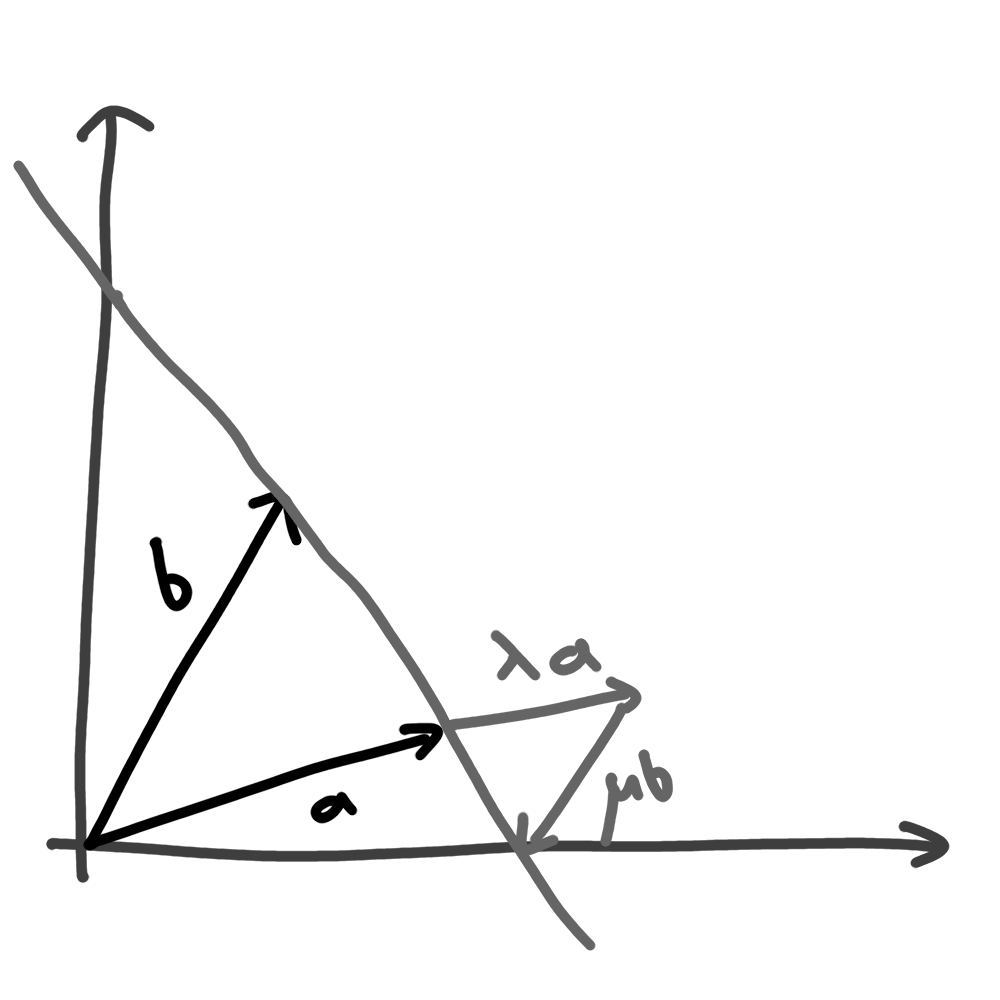
\includegraphics[width=0.3\linewidth]{figures/affine_combination_example}} 
		\subfigure{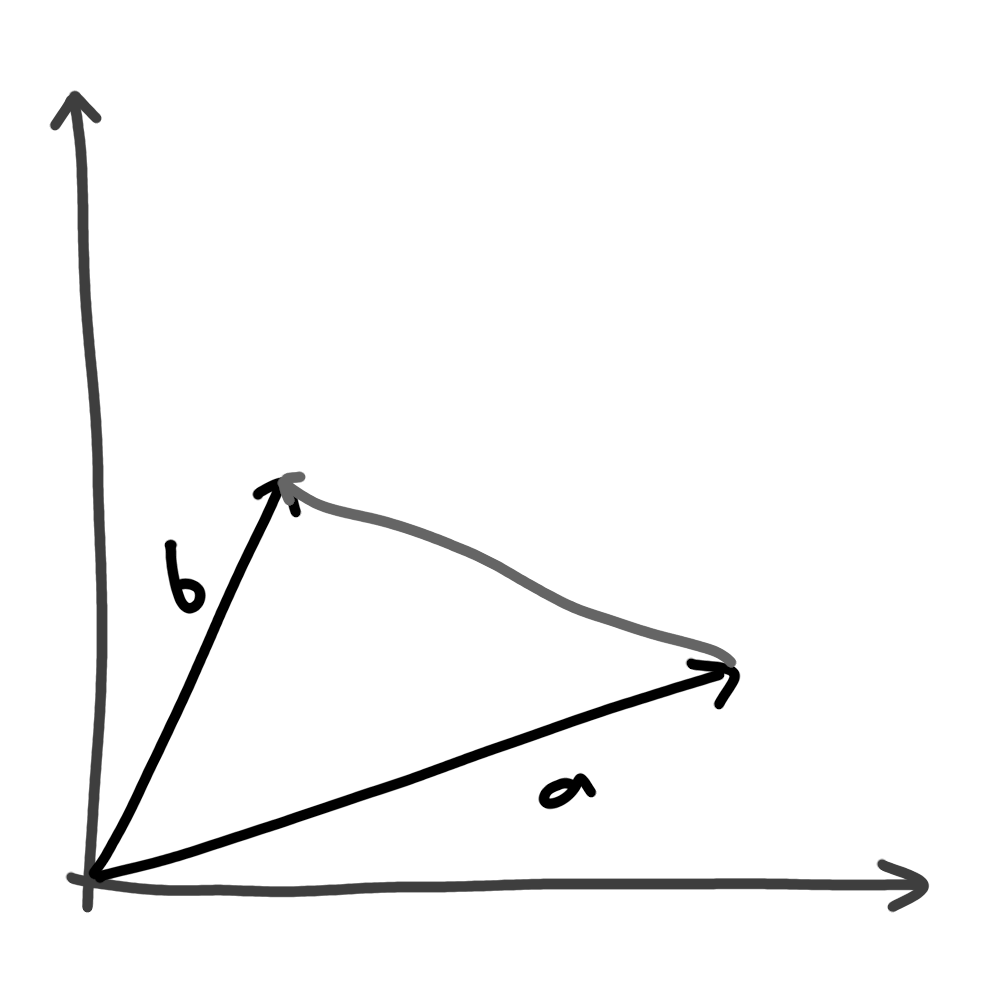
\includegraphics[width=0.3\linewidth]{figures/convex_combination_example}} 
		\caption{Linear combination, affine combination and convex combination}
		\label{fig:combinationexample}
	\end{figure}
	
	\textbf{Linear combination} $\lambda a + \mu b$

	\textbf{Affine combination} $\lambda a + \mu b$ and $\lambda + \mu = 1$
	
	What is $\mu$ so that $\lambda a + \mu B$ is on the line?
	\begin{align*}
		\lambda a + \mu b = a + t(b-a) \implies a (\underbrace{\lambda - 1 + t}_{=0}) + b (\underbrace{\mu - t}_{=0}) = 0
	\end{align*}
	If $a,b$ are linearly independent $\implies \mu = t \land \lambda + \mu = 1$

	\textbf{Convex combination} $\lambda a + \mu b$ and $\lambda + \mu = 1$ and $\lambda,\mu \geq 0$
	
	Line is $a + t(b-a)$ with $t\in[0,1]$ $\implies \mu,\lambda \in [0,1]$
\end{example}

\begin{definition}[combinations]
	linear combination $\sum_{i=1}^{n} \lambda_i v_i$ with $v_1,...,v_n \in \mathbb{R}^d, \lambda_1,...,\lambda_n \in \mathbb{R}$
	
	affine combination $\sum_{i=1}^{n} \lambda_i v_i$ with $\sum_{i=1}^{n} \lambda_i = 1$
	
	convex combination $\sum_{i=1}^{n} \lambda_i v_i$ with $\sum_{i=1}^{n} \lambda_i = 1$ and $\forall i: \lambda_i \geq 0$
\end{definition}

\begin{algorithm}[of de Casteljou, Bezier curve]
	Given: $b_0,...,b_n \in \mathbb{R}^d$ (called control points / Kontrollpunkte), $t \in \mathbb{R}$
	\\Recursion: $b_i^0(t) := b_i$
	\\$b_i^j(t) := (1-t)b_i^{j-1}(t) + tb_{i+1}^{j-1}(t)$ for $j=1,...,n$ and $i=0,...,n-j$
	\\Result: $b(t):=b_0^n(t)$ (called Bezier curve)
	
\end{algorithm}

\begin{remark}
	In the algorithm above often we choose $t\in[0,1]$.
\end{remark}

\begin{example}
	\begin{figure}[h!]
		\subfigure{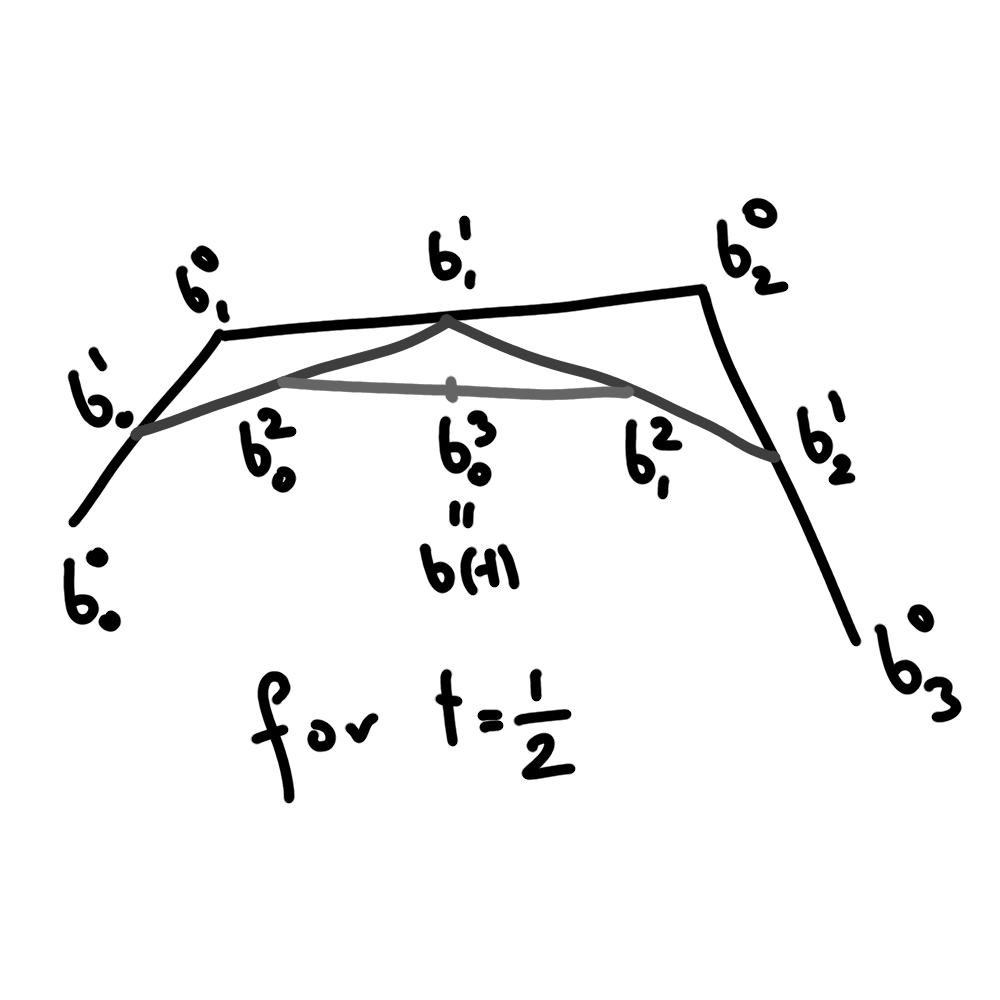
\includegraphics[width=0.3\linewidth]{figures/decasteljou_example_1}} 
		\subfigure{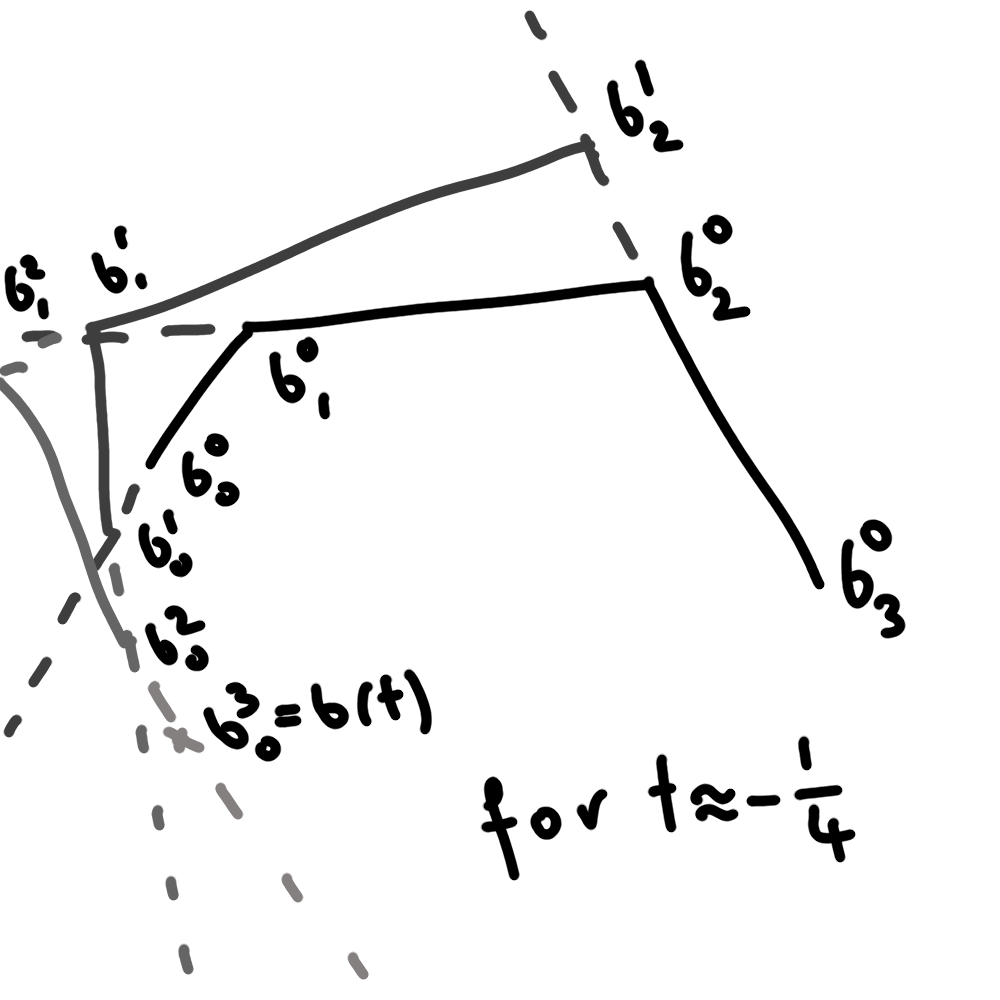
\includegraphics[width=0.3\linewidth]{figures/decasteljou_example_2}} 
		\subfigure{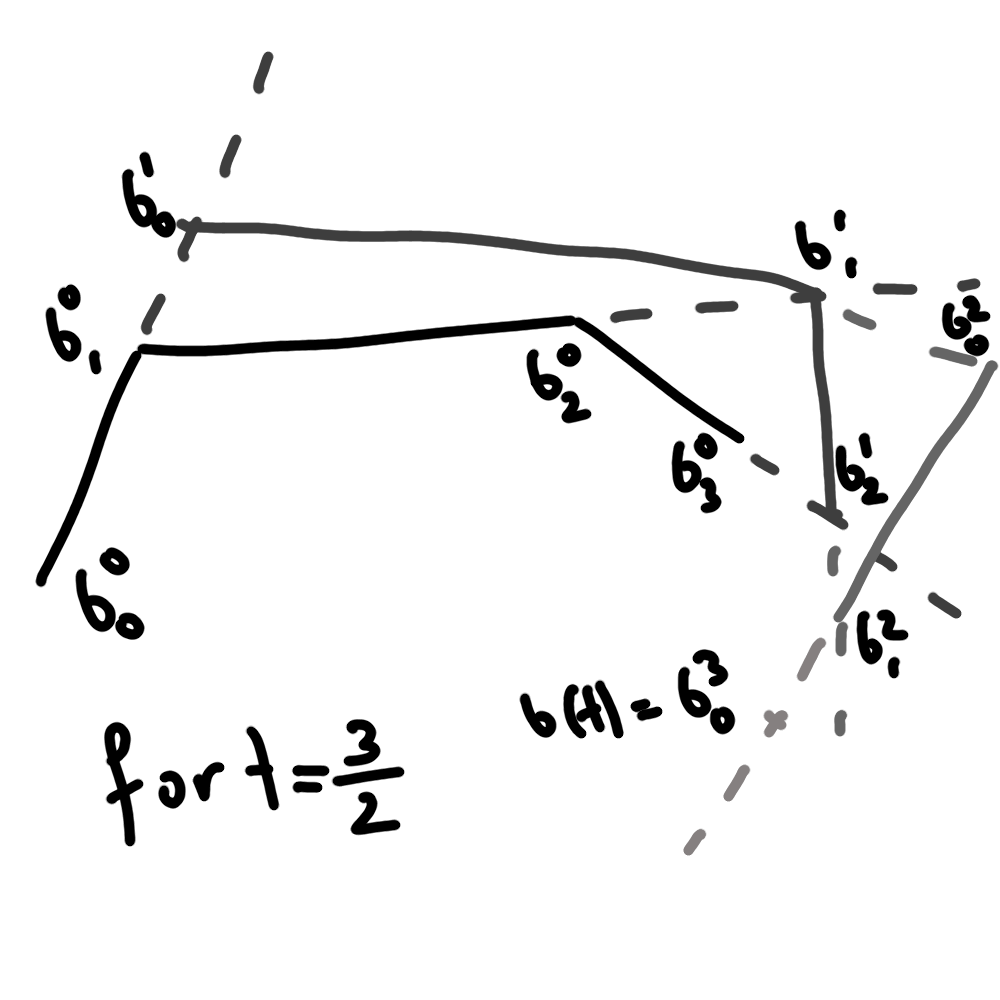
\includegraphics[width=0.3\linewidth]{figures/decasteljou_example_3}} 
		\caption{Examples of the de casteljou algorithm}
		\label{fig:decasteljouexample}
\end{figure}
\end{example}

\begin{remark}
	In this course $\mathbb{N}=\{1,2,3,...\}$ and $\mathbb{N}_0=\{0,1,2,3,...\}$
\end{remark}

\begin{recap}
	$0! := 1, n! := n(n-1)(n-2) \cdots 1$ for $n \geq 1$.
	
	\begin{align*}
		\binom{n}{k} := \begin{cases}
			\frac{n!}{k!(n-k)!}&, n\geq k \geq 0\\
			0&, k > n
		\end{cases} \text{ for } n,k \in \mathbb{N}_0
	\end{align*}
\end{recap}

\begin{definition}[Bernstein polynomials]
	For $n,i \in \mathbb{N}_0$ we define $B_i^n(t) := \binom{n}{i} t^i (1-t)^{n-i} \in \mathbb{R}[t]$
\end{definition}

\begin{remark}
	Special cases of Bernstein polynomials
	
	\begin{align*}
		i > n \implies B_i^n(t) = 0 && B_i^n(0) = \begin{cases}0, i\not= 0\\ 1, i=0 \end{cases} \\
		B_i^n(1) = \begin{cases}0, i\not= n\\ 1, i=n \end{cases} && B_0^0(t) = 1
	\end{align*}
\end{remark}

\begin{theorem}
	$b_i^j(t) = \sum_{l=0}^{j} B_l^j(t) b_{i+l}$
\end{theorem}

\begin{proof}
	Induction over $j$: $j=0$:
	\begin{align*}
		j=0: && b_i^0(t):= b_i = 1 \cdot b_i = B_0^0(t) \cdot b_i \hspace{1cm} \checkmark\\
		j-1 \rightarrow j: && b_i^j(t) := (1-t)b_i^{j-1}(t) + t b_{i+1}^{j-1}(t) \overset{\mathrm{IA}}{=}
		(1-t) \sum_{l=0}^{j-1} B_l^{j-1}(t) b_{i+l} + t \sum_{l=0}^{j-1} B_l^{j-1}(t) b_{i+1+l} =\\
		&& (1-t) \sum_{l=0}^{\overset{j}{\cancel{j-1}}} B_l^{j-1}(t) b_{i+l} + t \sum_{l=\underset{0}{\cancel{1}}}^{j} B_{l-1}^{j-1}(t) b_{i+l} =
		\sum_{l=0}^{j} (\underbrace{(1-t) B_l^{j-1}(t) + t B_{l-1}^{j-1}(t)}_{=B_l^j(t) \text{ using the following lemma}}) b_{i+l} =\\
		&& \sum_{l=0}^{j} B_l^j(t) b_{i+l} \hspace{1cm} \checkmark
	\end{align*}
\end{proof}

\begin{corollary}
	The Bezier curve equals $b(t) = b_0^n(t) = \sum_{l=0}^{n} B_l^j(t) b_{i+l}$, which is called the Bernstein representation of the Bezier curve.
\end{corollary}

\begin{remark}
	As $b(t) = \sum_{l=0}^{n} B_l^n(t) b_l \in C^\infty$ it is a polynomial curve of degree $n$, which is in $C^\infty$ and therefore ''very smooth''.
\end{remark}

\begin{lemma}
	$B_l^j(t) = (1-t)B_l^{j-1}(t) + t B_{l-1}^{j-1}(t)$
\end{lemma}

\begin{proof}
	\begin{align*}
		(1-t)B_l^{j-1}(t) + t B_{l-1}^{j-1}(t) = (1-t) \binom{j-1}{l} t^l (1-t)^{j-1-l} + t \binom{j-1}{l-1} t^{l-1} (1-t)^{j-1-l+1} =\\
		\binom{j-1}{l} t^l (1-t)^{j-l} + \binom{j-1}{l-1} t^{l} (1-t)^{j-l} = \left(\binom{j-1}{l} + \binom{j-1}{l-1}\right) t^l (1-t)^{j-l} = \binom{j}{l} t^l (1-t)^{j-l} = B_l^j(t)
	\end{align*}
\end{proof}

\begin{remark}
	What is $b(0)$? \hspace{1cm} $b(0)=\sum_{i=0}^{n} B_i^n(0) b_i = b_0 + 0 + 0 + \cdots + 0 = b_0$\\
	What is $b(1)$? \hspace{1cm} $b(1)=\sum_{i=0}^{n} B_i^n(1) b_i = 0 + \cdots + 0 + b_n = b_n$
\end{remark}

\begin{definition}[end-point-interpolating]
	Curves which pass through the first and last point are called end-point-interpolating (Endpunktinterpolierend).
\end{definition}

\begin{remark}
	Bezier curves are end-point-interpolating.
\end{remark}

\begin{remark}
	How many intersection points are there between a planar (i.e. in $\mathbb{R}^2$) Bezier curve and a straight line?
	\begin{align*}
		\text{Straight line: } p + t(q-p) && \text{ Bezier curve: } b(t) = \sum_{i=0}^{n} B_i^n(t) \underbrace{b_i}_{\in \mathbb{R}^2}
	\end{align*}
	
	Solving $p+t(q-p) = \sum_{i=0}^{n} B_i^n(t) b_i$ results in at most $n$ solutions.
\end{remark}

\begin{lemma}
	$\frac{d}{dt}B_i^n(t) = n(B_{i-1}^{n-1}(t) - B_i^{n-1}(t))$
\end{lemma}

\begin{proof}
	\begin{align*}
		\frac{d}{dt}B_i^n(t) = \frac{d}{dt} \binom{n}{i} t^i (1-t)^{n-i} = \binom{n}{i} i t^{i-1} (1-t)^{n-i} - \binom{n}{i} t^i (n-i) (1-t)^{n-i-1} =\\
		\frac{n!}{\underset{(i-1)!}{\cancel{i!}}(n-i)!} \cancel{i} t^{i-1} (1-t)^{n-i} - \frac{n!}{i!\underset{(n-i-1)!}{\cancel{(n-i)!}}}\cancel{(n-i)}t^i (1-t)^{n-i-1} =\\
		n \left(\frac{(n-1)!}{(i-1)!(n-i)!}t^{i-1}(1-t)^{n-i} - \frac{(n-1)!}{i!(n-i-1)!} t^i (1-t)^{n-i-1}\right) =\\
		n \left(\binom{n-1}{i-1}t^{i-1}(1-t)^{n-i} - \binom{n-1}{i} t^i (1-t)^{n-i-1}\right) = n(B_{i-1}^{n-1}(t) - B_i^{n-1}(t))
	\end{align*}
\end{proof}

\begin{theorem}
	$\dot{b}(t) := \frac{d}{dt} b(t) = n \sum_{i=0}^{n-1} B_i^{n-1}(t)(b_{i+1} - b_i) = n (b_1^{n-1}(t) - b_0^{n-1}(t))$
\end{theorem}

\begin{proof}
	\begin{align*}
		\dot{b}(t) = \frac{d}{dt} \left(\sum_{i=0}^{n} B_i^n(t) b_i\right) = \sum_{i=0}^{n} \frac{d}{dt} B_i^n(t) b_i = \sum_{i=0}^{n} n(B_{i-1}^{n-1}(t) - B_i^{n-1}(t)) b_i = n \left(\sum_{i=0}^{n} B_{i-1}^{n-1}(t) b_i - \sum_{i=0}^{n} B_i^{n-1}(t) b_i\right) =\\
		n \left(\sum_{i=1}^{n} B_{i-1}^{n-1}(t) b_i - \sum_{i=0}^{n} B_i^{n-1}(t) b_i\right) = n\left(\underbrace{\sum_{i=0}^{n-1} B_i^{n-1}(t) b_{i+1}}_{=b_1^{n-1}(t)} - \underbrace{\sum_{i=0}^{n-1} B_i^{n-1}(t) b_i}_{=b_0^{n-1}(t)}\right) = n \left(\sum_{i=0}^{n-1} B_i^{n-1}(t)(b_{i+1} - b_i)\right)
	\end{align*}
\end{proof}

\begin{corollary}
	\begin{itemize}
		\item $\dot{b}(0) = n (b_1 - b_0)$
		\item $\dot{b}(1) = n (b_n - b_{n-1})$
		\item The last segment in the algorithm of de Casteljou is the tangent of the Bezier curve in $b(t)$.
		\item The derivative of a bezier curve of degree $n$ is a bezier curve of degree $n-1$ with control points $(b_1,b_0), (b_2 - b_1), \cdots, (b_n - b_{n-1})$.
	\end{itemize}
\end{corollary}

\begin{corollary}
	$\ddot{b}(t) = n (n-1) \sum_{i=0}^{n-2} B_i^{n-2}(t) (b_{i+2} - 2 b_{i+1} + b_i)$
	
	$\ddot{b}(0) = n(n-1)(b_2 - 2b_1 + b_0)$, $\ddot{b}(1) = n(n-1)(b_n - 2b_{n-1} + b_{n-2})$
\end{corollary}

\begin{corollary}
	The curvature of a bezier curve in the point $b(0)$ depends only on $b_0, b_1, b_2$.
	
	The curvature of a bezier curve in the point $b(1)$ depends only on $b_{n-2}, b_{n-1}, b_n$.
\end{corollary}

\begin{example}
	Quadratic Bezier curve
	\begin{align*}
		b(t) = \sum_{i=0}^{2} B_i^2(t) b_i = \binom{2}{0} t^0 (1-t)^2 b_0 + \binom{2}{1} t^1 (1-t)^1 b_1 + \binom{2}{2} t^2 (1-t)^0 b_2 = t^2(b_2-2b_1+b_0) + t(2b_1 - 2b_0) + b_0
	\end{align*}
	which is an affine transformation of a parabola and therefore a parabola.
	
	Quadratic bezier curves are parabolas.
\end{example}

\begin{remark}
	Line at infinity (Ferngerade) is the collection of points where parallel lines intersect.
	
	\begin{figure}[h!]
		\centering
		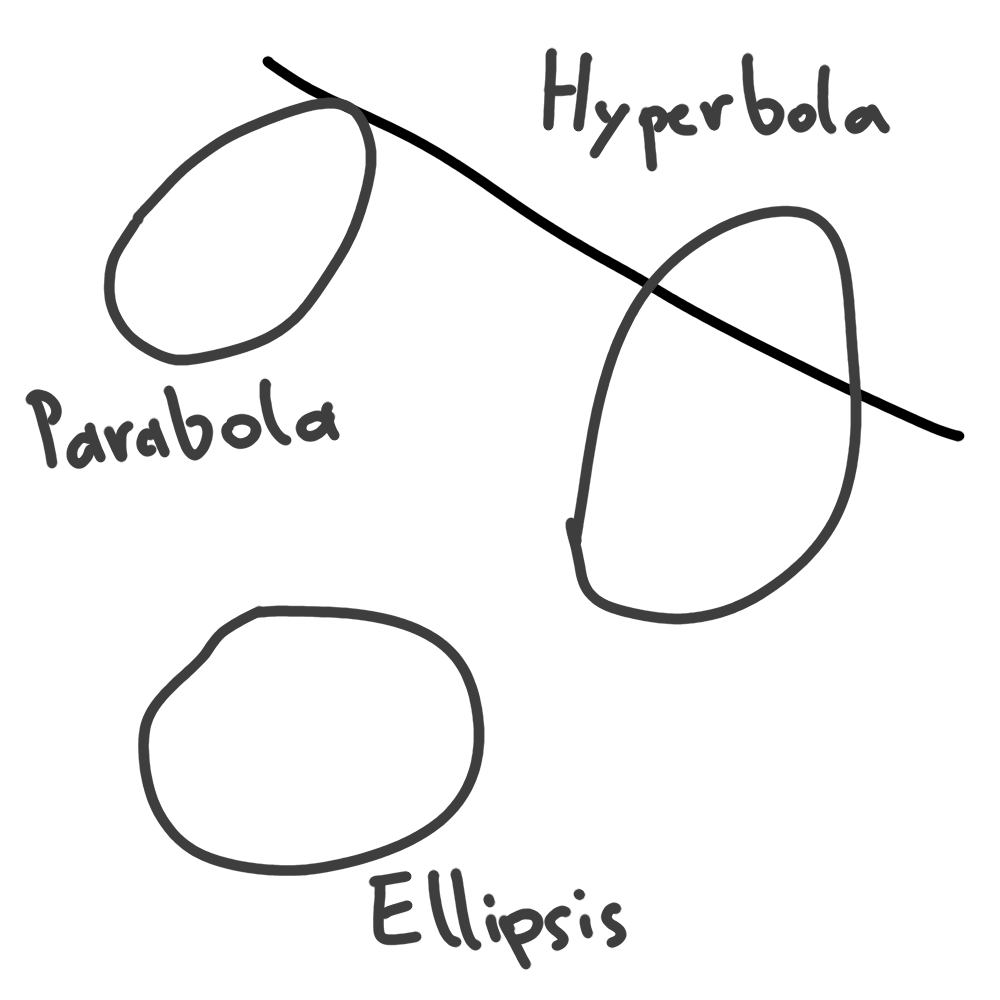
\includegraphics[width=0.3\linewidth]{figures/line_at_infinity}
		\caption{Categorization of Parabolas, Hyperbolas and Ellipsis as intersection points with the line at infinity.}
		\label{fig:lineatinfinity}
	\end{figure}
	
\end{remark}

\begin{remark}
	Different applications using these curves are Rhino, OpenSCAD, Autocad, Geogebra, ...
\end{remark}



\section{Parameterized curves}

\begin{figure}[h!]
	\centering
	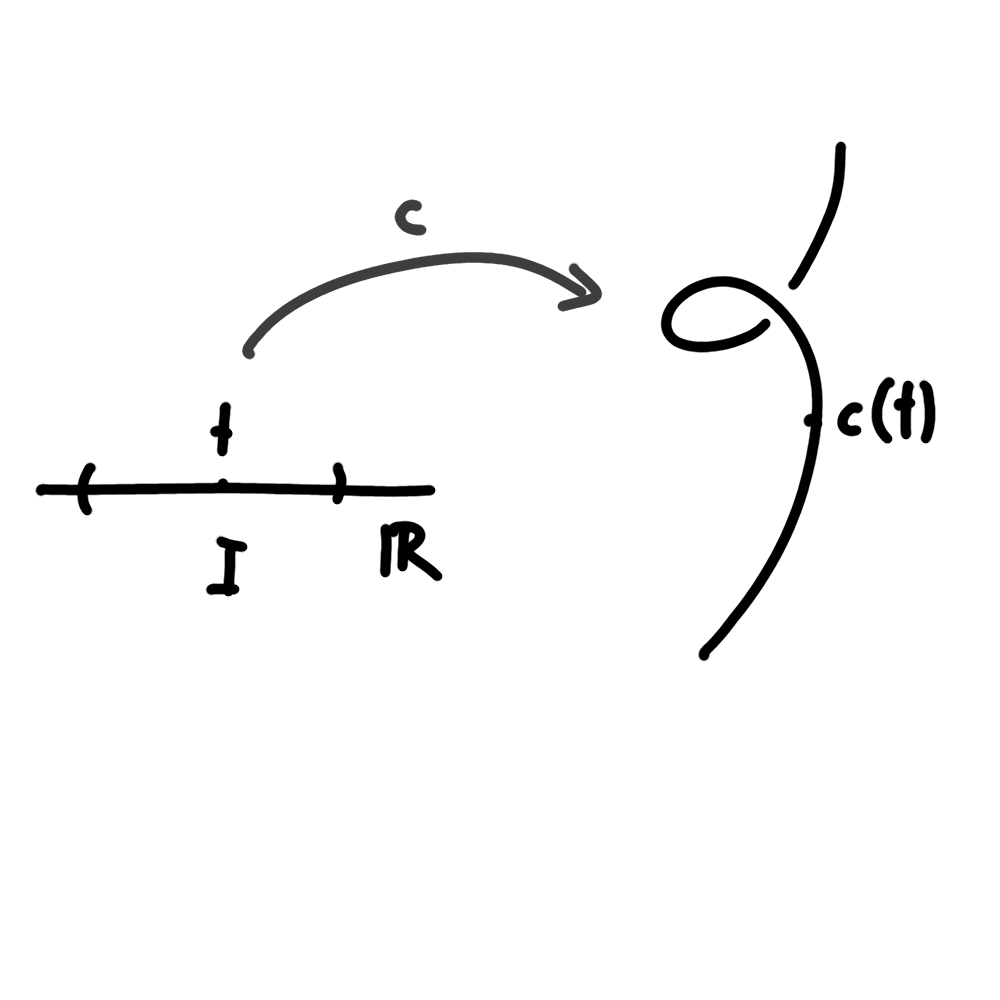
\includegraphics[width=0.3\linewidth]{figures/parameterized_curve}
	\caption{parameterized curve $c(t)$}
	\label{fig:parameterizedcurve}
\end{figure}

\begin{definition}
	$c:I\subseteq \mathbb{R} \rightarrow \mathbb{R}^3$ is called a parameterized curve.
	 
	
	$\dot{c}(t) := \frac{d}{dt} c(t)$ is called the tangential vector. For $\mathbb{R}^3$ we have $\dot{c}(t) = (\dot{c_1}(t), \dot{c_2}(t), \dot{c_3}(t))$.

	The velocity is defined as $|| \dot{c}(t) ||$.
	
	A point $c(t)$ is called regular, if $\dot{c}(t) \not= 0$ and is called singular, if $\dot{c}(t) = 0$.
\end{definition}

\begin{example}
	A helix (Schraublinie) is defined by $c(t) = (\cos(t), \sin(t), t)^T$.
	
	\begin{figure}[h!]
		\centering
		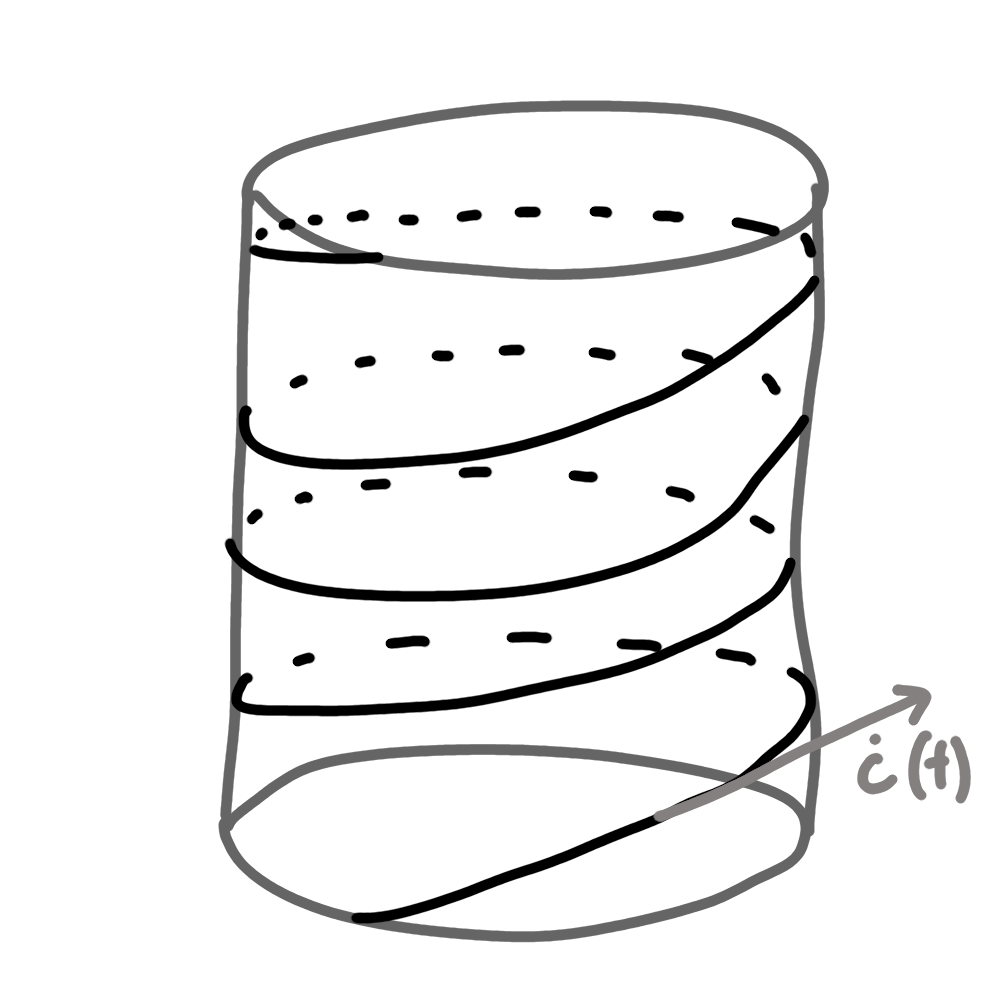
\includegraphics[width=0.3\linewidth]{figures/helix}
		\caption{Helix with tangential vector}
		\label{fig:helix}
	\end{figure}
	
	\begin{align*}
		\dot{c}(t) = (-\sin(t), \cos(t), 1)^T && ||\dot{c}(t)|| = \sqrt{\sin^2(t) + \cos^2(t) + 1} = \sqrt{2}
	\end{align*}
	
	We see that the helix is passed through with constant velocity. Furthermore all points are regular.
\end{example}

\begin{example}
	$c:\mathbb{R} \rightarrow \mathbb{R}^3, t \mapsto (t^2, t^3, t^4)$, $\dot{c}(t) = (2t, 3t^2, 4t^3)$. We see that $0$ is singular as $\dot{c}(0) = (0, 0, 0)$. Everywhere else the curve is regular.
\end{example}

\begin{remark}
	A point being regular or singular depends on the parameterisation of the curve.
	
	For example $c(t) = (t,t)$ produces a regular curve, while $c(t) = (t^3, t^3)$ produces a curve where $0$ is singular.
	
	
	\begin{figure}[h!]
		\centering
		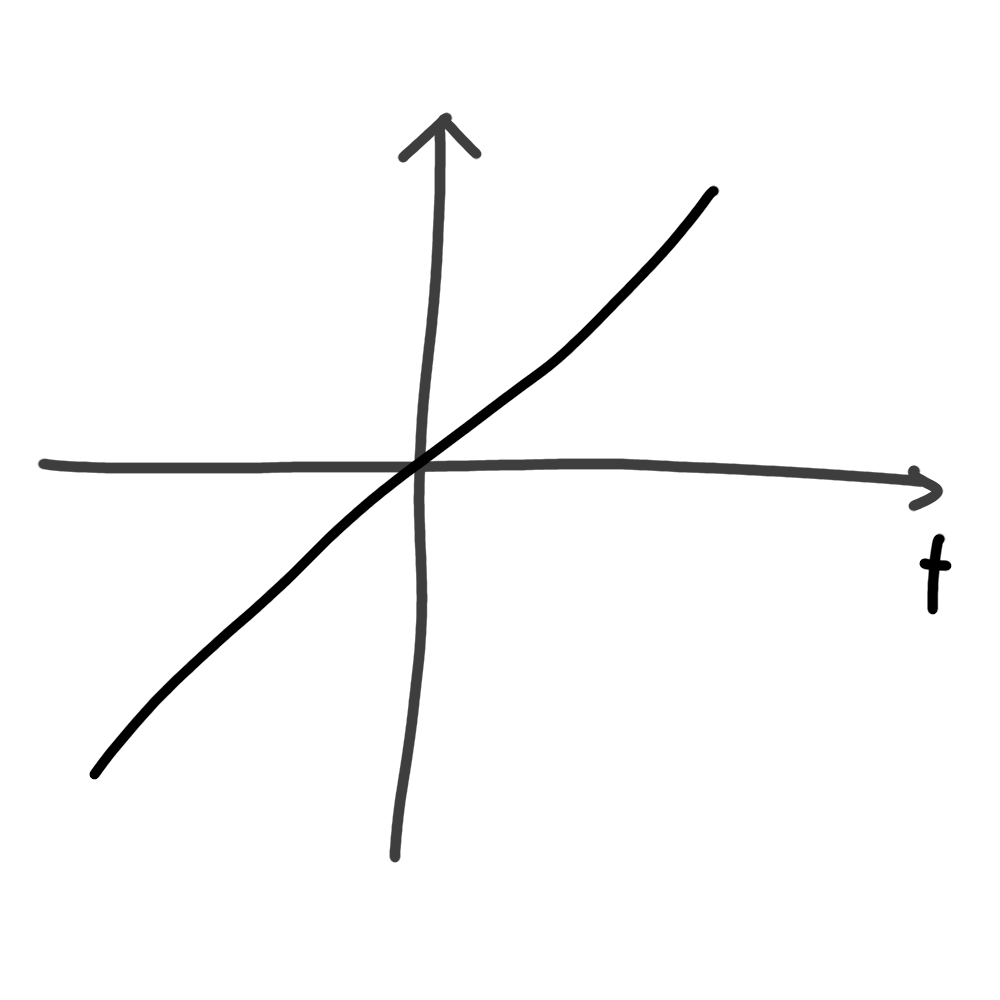
\includegraphics[width=0.3\linewidth]{figures/identity_line}
		\caption{identity line can be parameterized such that $(0, 0)$ is singular.}
		\label{fig:identityline}
	\end{figure}
	
	
	There are curves and points where no parameterisation exists such that the point is regular.	
\end{remark}

\begin{definition}
	$c: I \rightarrow \mathbb{R}^2 \in C^2(I, \mathbb{R}^2)$
	
	The curvature of the curve in the point $c(t)$ is defined as $\kappa(t) = \frac{\det(\dot{c}(t), \ddot{c}(t))}{||\dot{c}(t)||^3}$
\end{definition}

\begin{example}
	\begin{figure}[h!]
		\centering
		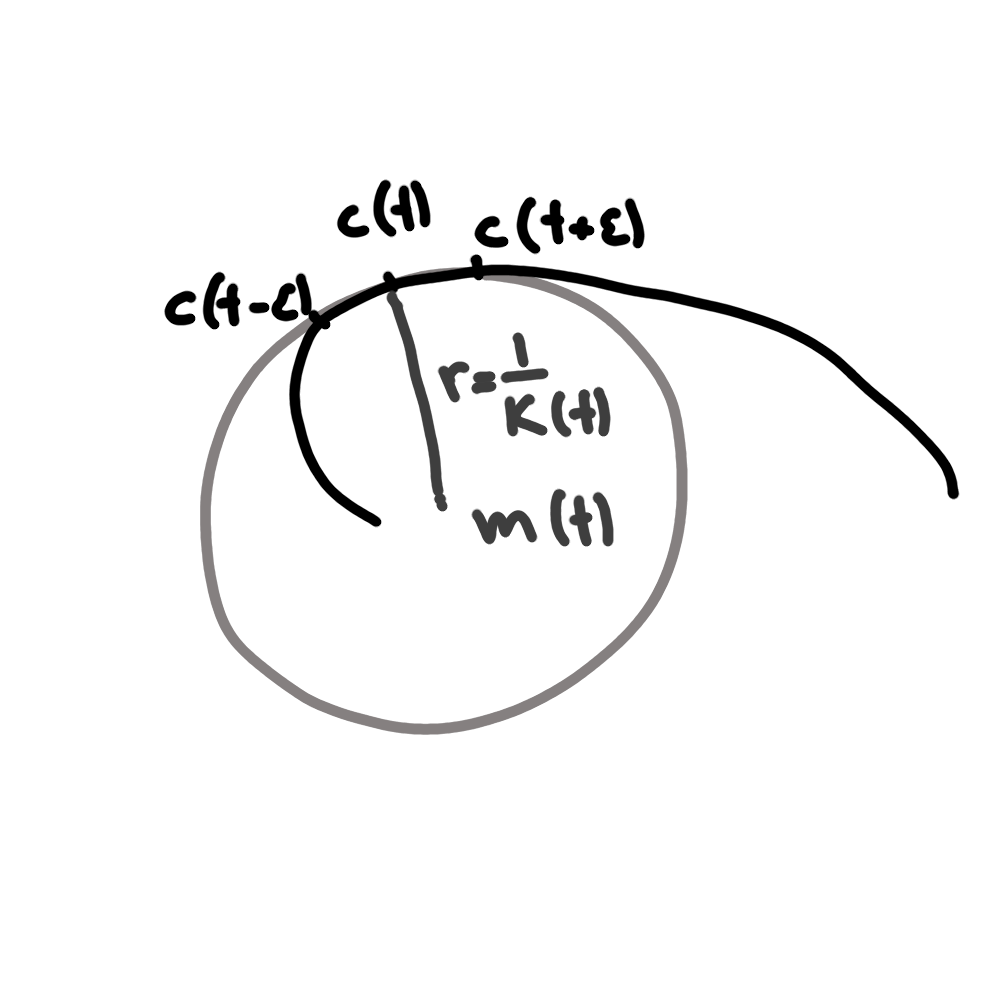
\includegraphics[width=0.3\linewidth]{figures/circle_of_curvature}
		\caption{Circle of curvature}
		\label{fig:circleofcurvature}
	\end{figure}
	
	The circle of curvature has a radius of $\frac{1}{\kappa(t)}$. $m(t)$ is called the center of curvature.
	
	$m(t) = c(t) + \frac{1}{\kappa(t)}n(t)$ where $n(t) = \frac{(-\dot{c_2}(t), \dot{c_1}(t))}{||\dot{c}(t)||}$.
\end{example}

\begin{remark}
	Exercise: compare this definition of curvature with the school version concerning graphs.
\end{remark}

\begin{example}
	For a circle we have $c(t) = (r\cos(t), r\sin(t))^T$, $\dot{c}(t) = (-r\sin(t), r\cos(t))^T$, $\ddot{c}(t) = (-r\cos(t), -r\sin(t))^T$
	
	\begin{align*}
		\kappa(t) = \frac{\det \left(\begin{matrix}
				-r \sin(t) & -r \cos(t) \\
				r \cos(t) & -r \sin(t)
		\end{matrix}\right) }{r^3} = \frac{r^2\sin^2(t) + r^2\cos^2(t)}{r^3} = \frac{r^2}{r^3} = \frac{1}{r}\\
		n(t) = \frac{(-r \cos(t), -r \sin(t))}{r} = (-\cos(t), -\sin(t))
	\end{align*}
	
	\begin{figure}[h!]
		\centering
		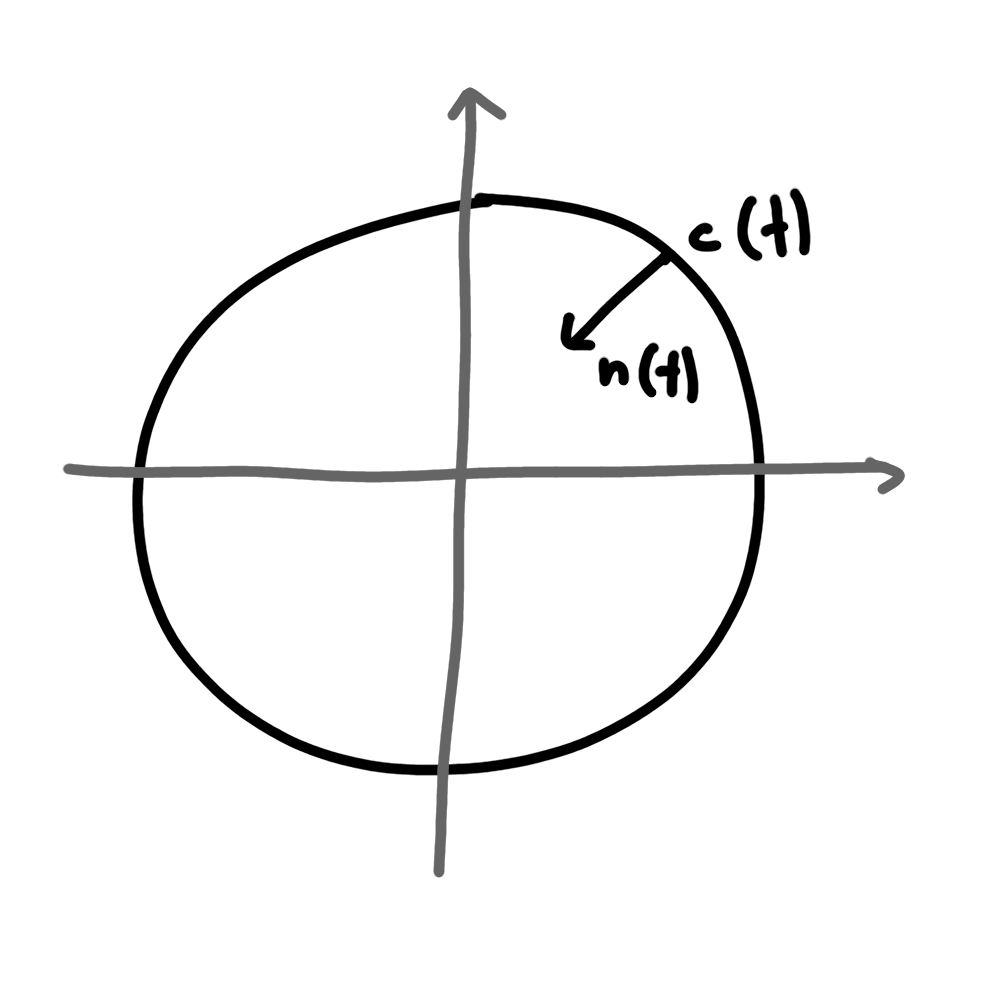
\includegraphics[width=0.3\linewidth]{figures/circle_with_normal_vector}
		\caption{Circle with normal vector}
		\label{fig:circlewithnormalvector}
	\end{figure}
	
\end{example}

\begin{definition}
	A point $c(t)$ with $\dot{\kappa}(t) = 0$ is called a vertex.
\end{definition}

\begin{example}
	An ellipse has four vertices.
	
	\begin{figure}[h!]
		\centering
		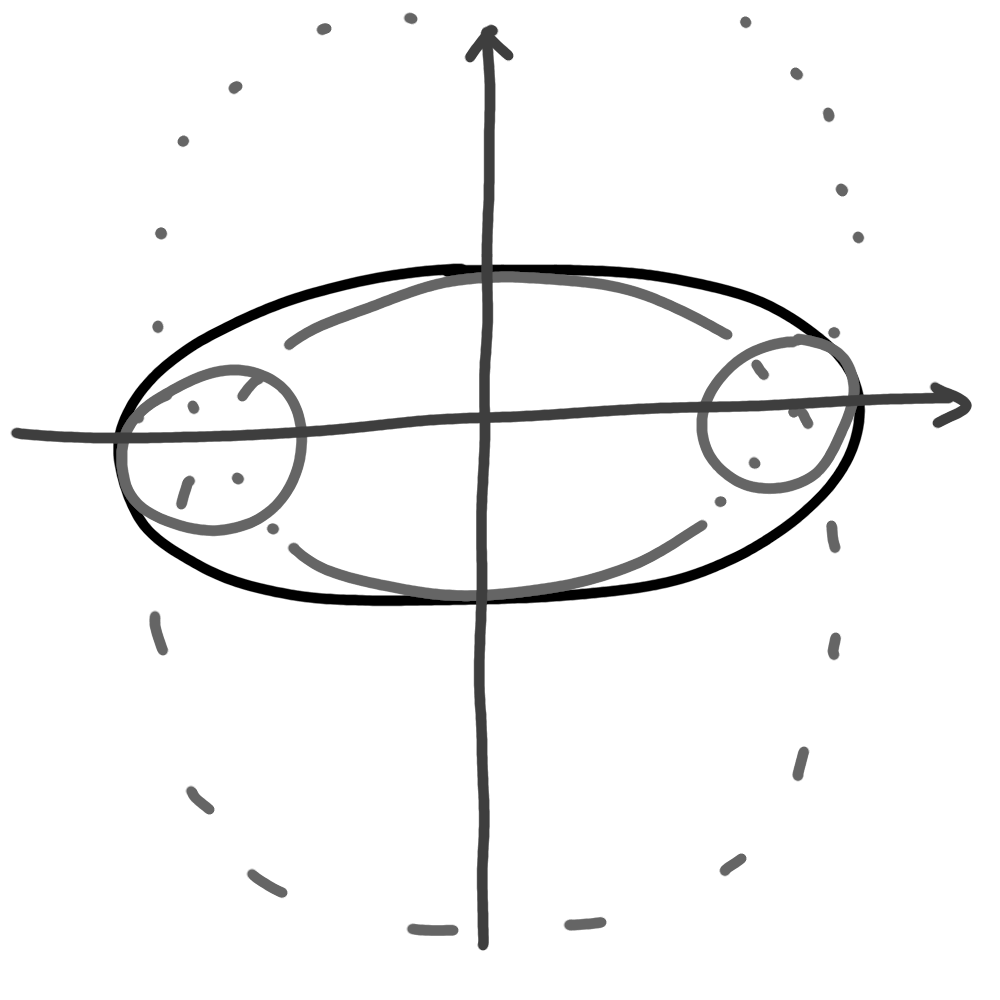
\includegraphics[width=0.3\linewidth]{figures/ellipse}
		\caption{Ellipse and the four vertices.}
		\label{fig:ellipse}
	\end{figure}
	
	
	$(t, \exp t)$ has no vertex.
	
	Klothoids are curves with $\kappa(t) = t$. They are used in road construction and have no vertex.
\end{example}

\begin{definition}
	$c:I \rightarrow \mathbb{R}^3$
	
	$\kappa(t) = \frac{||\dot{c}(t) \times \ddot{c}(t)||}{||\dot{c}(t)||^3}$ is called the curvature of a space curve.
	
	$\tau(t) = \frac{\det (\dot{c}(t), \ddot{c}(t), \dddot{c}(t))}{||\dot{c}(t) \times \ddot{c}(t)||^2}$ is called torsion of a space curve.
\end{definition}

\begin{example}
	For the helix $t \mapsto (\cos(t), \sin(t), pt)$ the torsion depends on $p$.	
\end{example}

\section{Properties of Bezier curves}

\begin{definition}
	$\alpha: \mathbb{R}^n \rightarrow \mathbb{R}^m$ is called \textbf{affine} if $\exists l:\mathbb{R}^n \rightarrow \mathbb{R}^m$...linear $\exists v \in \mathbb{R}^m: \alpha(x) = l(x) + v$.
	
	$\alpha$ is called \textbf{affinity} if $\alpha$ is affine and bijective.
\end{definition}

\begin{example}
	An example of an linear function is shear (Scherung).
	\begin{align*}
		l\left(\begin{matrix} x \\ y \end{matrix}\right) := \left(\begin{matrix} 1 & a \\ 0 & 1 \end{matrix}\right) \left(\begin{matrix} x\\ y \end{matrix}\right)
	\end{align*}
	
	Area is preserved.
\end{example}

\end{document}
